\chapter{Elekrizitätslehre}
zuerst Elektrostatik!

\section{Elektrostatik}
\subsection{Das Elektrische Feld}
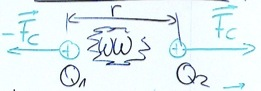
\includegraphics{Bild147} \\
\[
	F_C = \frac{1}{4 \pi \epsilon_0} \frac{Q_1 Q_2}{r^2} \\
	\epsilon_0 = \SI{8.85E-12}{\ampere\second\per\volt\metre}
\]
\uline{hier:} \\
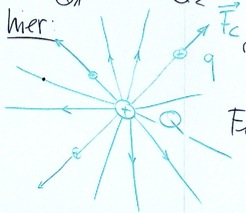
\includegraphics{Bild148}
\begin{def*}[ note = elektrische Feld , index = elektrische Feld , indexformat = {1!~2 2!1~} ]
	\[ \boxed{ \vec{E} = \frac{\vec{F_C}}{q} } \]
\end{def*}
\uline{hier:}
\[ E = \frac{1}{4 \pi \epsilon_0} \frac{Q}{r^2} \]
für Punktladung

\subsubsection{Feldlinien}
\begin{itemize}
	\item $\vec{E}$ tangential zu FL \\
		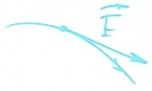
\includegraphics{Bild149}
	\item Richtungssinn!
	\item Dichte der FL $\sim \abs{\vec{E}(\vec{r})}$
	\item Vorzeichen: \\
		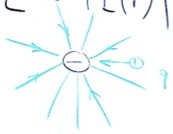
\includegraphics{Bild150}
\end{itemize}

\subsubsection{Mehrere Punktladungen}
\begin{bsp*}
	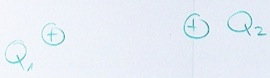
\includegraphics{Bild151} \\
	\uline{Vektoraddition!} \\
	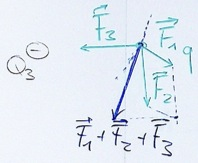
\includegraphics{Bild152}
\end{bsp*}

\subsubsection{Das Dipolfeld}
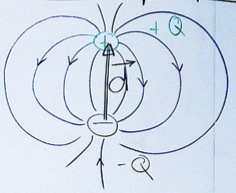
\includegraphics{Bild153}
\begin{def*}[ note = Dipolmoment , index = Dipolmoment ]
	\[ \boxed{ \vec{p} = Q \cdot \vec{d} } \]
	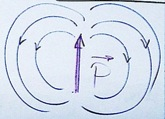
\includegraphics{Bild154}
\end{def*}

\subsubsection{Dipol in äusserem Feld}
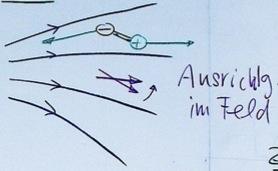
\includegraphics{Bild155} \\
\begin{itemize}
	\item Drehmoment
	\item Kraft (inhomogenes Feld)
\end{itemize}
\begin{bsp*}[ head = z.B. , note = \ce{H2O}-Molekül ]
	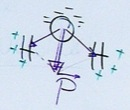
\includegraphics{Bild156}
\end{bsp*}

\subsubsection{Homogenes \texorpdfstring{$\vec{E}$}{E}-Feld}
\subsubsection{Plattenkondensator}
(kontinuierliche Ladungsverteilung) \\
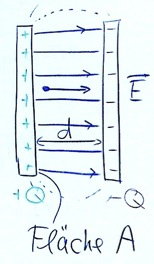
\includegraphics{Bild157} \\
Im Innern:
\[ \boxed{ E = \frac{Q}{\epsilon_0 A} } \]
Aussen: $E \approx 0$

\subsection{Die Elektrische Spannung}
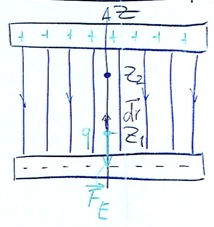
\includegraphics{Bild158} \\
Arbeit von \uline{mir}
\[
	W_{1 \rightarrow 2} = \int_{z_1}^{z_2} \vec{F} \cdot \vec{\dd r} = q E ( z_2 - z_1 ) > 0 \\
	( \vec{F} = - \vec{\overline{F_E}} = - q \vec{E} = \text{ konst. } )
\]
\begin{def*}[ note = elektrische Spannung , index = elektrische Spannung , indexformat = {1!~2 2!1~} ]
	\[
		\boxed{ U_{21} = \frac{W_{1 \rightarrow 2}}{q} }
		\intertext{( = Arbeit / Ladung )}
		[ U ] = \si{\joule\per\coulomb} = \si{\volt}
	\]
\end{def*}

\begin{rep*}[ note = Die elektrische Spannung ]
	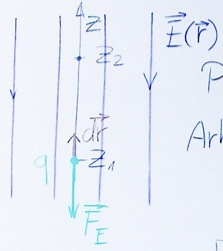
\includegraphics{Bild159} \\
	\[
		\vec{E}(\vec{r}) \text{ hier homogen} \\
		\text{Probeladung } q \\
		\text{Arbeit } W_{1 \rightarrow 2} = \int_{z_1}^{z_2} \underbrace{\vec{F}}_{\text{\enquote{meine Kraft} } \vec{F} = - \vec{F_E} = - q \cdot E} \cdot \vec{\dd r} = q \cdot E ( z_2 - z_1 )
	\]
	\begin{def*}[ note = Spannung , index = Spannung ]
		\[ U_{21} = \frac{W_{1 \rightarrow 2}}{q} \]
	\end{def*}
\end{rep*}

konservatives Kraftfeld
\begin{itemize}[ label = $\implies$ ]
	\item $W_{1 \rightarrow 2}$ unabhängig vom Weg
	\item $W_{1 \rightarrow 2} = E_{\text{pot}}(z_2) - E_{\text{pot}}(z_1)$
\end{itemize}
Das \textbf{elektrische Potential}
\[ \boxed{ \phi(x) = \frac{E_{\text{pot}}(z)}{q} } \]
$\implies U_{21} = \phi(z_2) - \phi(z_1)$ \\
Spannung = Potenitaldifferenz
\begin{bsp*}
	hier $W_{1 \rightarrow 2} > 0$ \\
	$z_2$ liegt auf höherem Potential
\end{bsp*}

\subsection{Bewegung \texorpdfstring{$\perp$}{senkrecht zum} \texorpdfstring{$\vec{E}$}{E}-Feld}
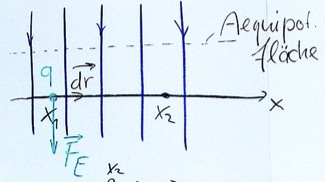
\includegraphics{Bild160}
\[ \begin{split}
	W_{1 \rightarrow 2}
		&= \int_{x_1}^{x_2} \vec{F} \cdot \vec{\dd r} = 0 \\
		&= U_{21} = 0 \\
		&= \phi(x_2) - \phi(x_1)
\end{split} \]
\begin{bsp*}[ note = Plattenkondensator ]
	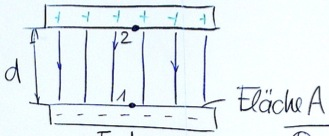
\includegraphics{Bild161}
	\[ U_{21} = - \frac{qEd}{q} = \underbrace{Ed}_{E = \frac{Q}{\epsilon_0 A}} = \frac{Qd}{\epsilon_0 A} \]
	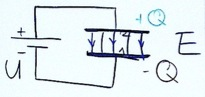
\includegraphics{Bild162}
	\[ U_{21} = U \implies E = \frac{U}{d} \quad \left[ \si{\volt\per\metre} \right] \]
\end{bsp*}
\begin{def*}[ note = Kapazität , index = Kapazität ]
	\[ C = \frac{Q}{U} \]
	
	\[ \text{Plattenkondensator } C = \frac{\epsilon_0 A}{d} \]
\end{def*}

\subsubsection{Beliebiges \texorpdfstring{$\vec{E}$}{E}-Feld}
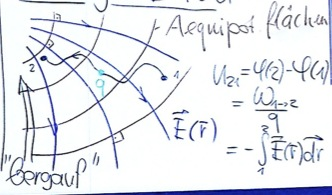
\includegraphics{Bild163}
\[ \begin{split}
	U_{21}
		&= \phi(2) - \phi(1) \\
		&= \frac{W_{1 \rightarrow 2}}{q} \\
		&= - \int_{1}^{2} \vec{E}(\vec{r}) \vec{\dd r}
\end{split} \]

\subsubsection{Beschleunigung in Röntgenröhre}
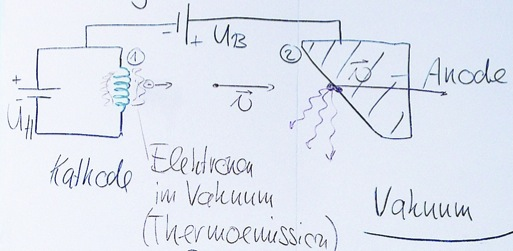
\includegraphics{Bild164}
\[
	\left. \begin{matrix*}[l]
		\phi(2) > \phi(1) \\
		q = -e
	\end{matrix*} \right\} \quad E_{\text{pot}}(2) < E_{\text{pot}}(1) \\
	\text{EEH: } -e \phi(1) + \underbrace{\frac{1}{2} m v_1^2}_{0} = -e \phi(2) + \frac{1}{2} m v_2^2 \\
	\implies \frac{1}{2} m v_2^2 = e ( \phi(2) - \phi(1) ) = e \cdot U_B
\]

\subsubsection{Materialien in elektrischen Feldern}
\subsubsection{Metalle}
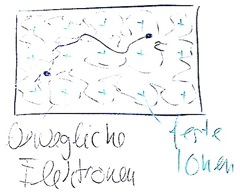
\includegraphics{Bild165} \\
laden \\
\begin{tabular}{ l l }
	$+Q$ &Elektronen weg \\
	$-Q$ &Elektronen dazu
\end{tabular}

\subsubsection{Isolator}
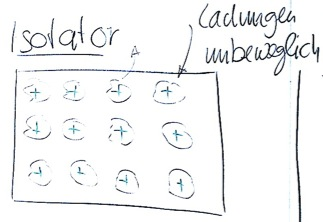
\includegraphics{Bild166}

\subsubsection{Metalle}
Elektrostatik $\vec{v} = \vec{0}$
\begin{itemize}[ label = $\implies$ ]
	\item im Innern $\vec{E} = \vec{0}$
	\item Metalle sind Aequipotentialgebiete
\end{itemize}
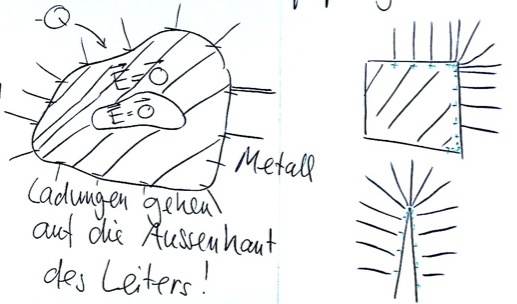
\includegraphics{Bild167}

\subsubsection{Metall in äusserem Feld}
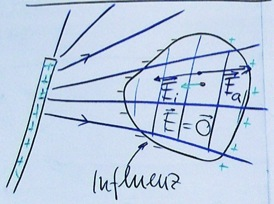
\includegraphics{Bild168} \\
Elektrometer \\
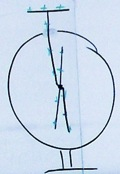
\includegraphics{Bild169}

\subsubsection{Isolator im äusseren Feld}
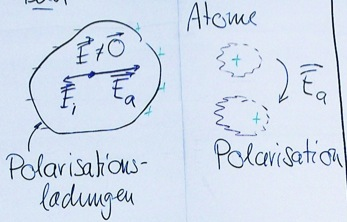
\includegraphics{Bild170}

\subsection{Elektrische Gleichströme: Leiter}
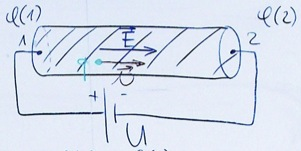
\includegraphics{Bild171} \\
\begin{itemize}[ label = $\implies$ ]
	\item $\phi(1) > \phi(2)$
	\item keine Aequipotentialfläche
\end{itemize}
$\vec{E}$-Feld beschleunigt Ladungen \\
Reibung an Ionen bremst sie \\
$\implies \vec{v} =$ konst.












